E' stata fatta la simulazione per la risposta in frequenza utilizzando Spice, con l'accortezza di scaricare la libreria del componente
dal sito della Texas Instrument.
I  \autoref{gr:sim_a5.tex} e \autoref{gr:sim_a10.tex} mostrano il confronto della simulazione con 
i dati sperimentali e mostrano un buon accordo tra i dati e la simulazione.
Nel \autoref{gr:sim_a1.tex}, relativo all'ampificazione A=1, si nota una deviazione dei dati sperimentali dovuta alla risonanza,
causata dalle induttanze parassite nel circuito reale, che comportano lo spostamento verso le basse frequenze del polo.

\begin{grafico}
 \centering
 \resizebox{\textwidth}{!}{%
 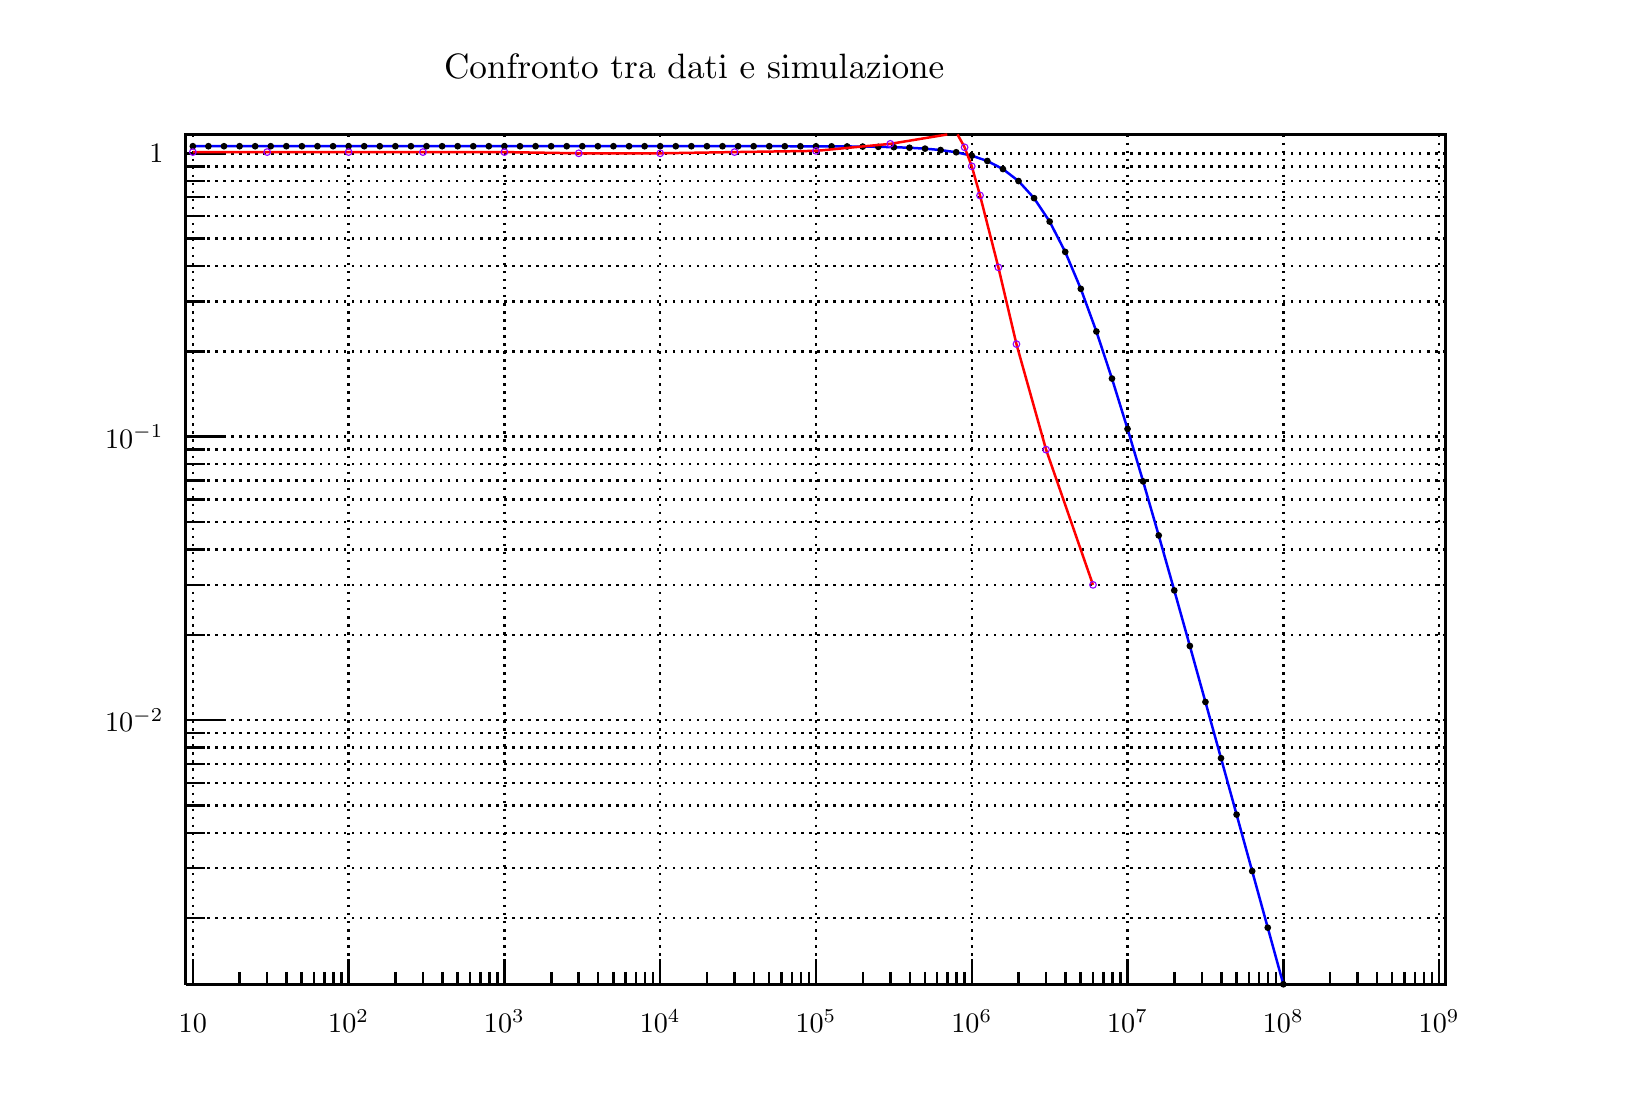
\begin{tikzpicture}
\pgfdeclareplotmark{cross} {
\pgfpathmoveto{\pgfpoint{-0.3\pgfplotmarksize}{\pgfplotmarksize}}
\pgfpathlineto{\pgfpoint{+0.3\pgfplotmarksize}{\pgfplotmarksize}}
\pgfpathlineto{\pgfpoint{+0.3\pgfplotmarksize}{0.3\pgfplotmarksize}}
\pgfpathlineto{\pgfpoint{+1\pgfplotmarksize}{0.3\pgfplotmarksize}}
\pgfpathlineto{\pgfpoint{+1\pgfplotmarksize}{-0.3\pgfplotmarksize}}
\pgfpathlineto{\pgfpoint{+0.3\pgfplotmarksize}{-0.3\pgfplotmarksize}}
\pgfpathlineto{\pgfpoint{+0.3\pgfplotmarksize}{-1.\pgfplotmarksize}}
\pgfpathlineto{\pgfpoint{-0.3\pgfplotmarksize}{-1.\pgfplotmarksize}}
\pgfpathlineto{\pgfpoint{-0.3\pgfplotmarksize}{-0.3\pgfplotmarksize}}
\pgfpathlineto{\pgfpoint{-1.\pgfplotmarksize}{-0.3\pgfplotmarksize}}
\pgfpathlineto{\pgfpoint{-1.\pgfplotmarksize}{0.3\pgfplotmarksize}}
\pgfpathlineto{\pgfpoint{-0.3\pgfplotmarksize}{0.3\pgfplotmarksize}}
\pgfpathclose
\pgfusepathqstroke
}
\pgfdeclareplotmark{cross*} {
\pgfpathmoveto{\pgfpoint{-0.3\pgfplotmarksize}{\pgfplotmarksize}}
\pgfpathlineto{\pgfpoint{+0.3\pgfplotmarksize}{\pgfplotmarksize}}
\pgfpathlineto{\pgfpoint{+0.3\pgfplotmarksize}{0.3\pgfplotmarksize}}
\pgfpathlineto{\pgfpoint{+1\pgfplotmarksize}{0.3\pgfplotmarksize}}
\pgfpathlineto{\pgfpoint{+1\pgfplotmarksize}{-0.3\pgfplotmarksize}}
\pgfpathlineto{\pgfpoint{+0.3\pgfplotmarksize}{-0.3\pgfplotmarksize}}
\pgfpathlineto{\pgfpoint{+0.3\pgfplotmarksize}{-1.\pgfplotmarksize}}
\pgfpathlineto{\pgfpoint{-0.3\pgfplotmarksize}{-1.\pgfplotmarksize}}
\pgfpathlineto{\pgfpoint{-0.3\pgfplotmarksize}{-0.3\pgfplotmarksize}}
\pgfpathlineto{\pgfpoint{-1.\pgfplotmarksize}{-0.3\pgfplotmarksize}}
\pgfpathlineto{\pgfpoint{-1.\pgfplotmarksize}{0.3\pgfplotmarksize}}
\pgfpathlineto{\pgfpoint{-0.3\pgfplotmarksize}{0.3\pgfplotmarksize}}
\pgfpathclose
\pgfusepathqfillstroke
}
\pgfdeclareplotmark{newstar} {
\pgfpathmoveto{\pgfqpoint{0pt}{\pgfplotmarksize}}
\pgfpathlineto{\pgfqpointpolar{44}{0.5\pgfplotmarksize}}
\pgfpathlineto{\pgfqpointpolar{18}{\pgfplotmarksize}}
\pgfpathlineto{\pgfqpointpolar{-20}{0.5\pgfplotmarksize}}
\pgfpathlineto{\pgfqpointpolar{-54}{\pgfplotmarksize}}
\pgfpathlineto{\pgfqpointpolar{-90}{0.5\pgfplotmarksize}}
\pgfpathlineto{\pgfqpointpolar{234}{\pgfplotmarksize}}
\pgfpathlineto{\pgfqpointpolar{198}{0.5\pgfplotmarksize}}
\pgfpathlineto{\pgfqpointpolar{162}{\pgfplotmarksize}}
\pgfpathlineto{\pgfqpointpolar{134}{0.5\pgfplotmarksize}}
\pgfpathclose
\pgfusepathqstroke
}
\pgfdeclareplotmark{newstar*} {
\pgfpathmoveto{\pgfqpoint{0pt}{\pgfplotmarksize}}
\pgfpathlineto{\pgfqpointpolar{44}{0.5\pgfplotmarksize}}
\pgfpathlineto{\pgfqpointpolar{18}{\pgfplotmarksize}}
\pgfpathlineto{\pgfqpointpolar{-20}{0.5\pgfplotmarksize}}
\pgfpathlineto{\pgfqpointpolar{-54}{\pgfplotmarksize}}
\pgfpathlineto{\pgfqpointpolar{-90}{0.5\pgfplotmarksize}}
\pgfpathlineto{\pgfqpointpolar{234}{\pgfplotmarksize}}
\pgfpathlineto{\pgfqpointpolar{198}{0.5\pgfplotmarksize}}
\pgfpathlineto{\pgfqpointpolar{162}{\pgfplotmarksize}}
\pgfpathlineto{\pgfqpointpolar{134}{0.5\pgfplotmarksize}}
\pgfpathclose
\pgfusepathqfillstroke
}
\definecolor{c}{rgb}{1,1,1};
\draw [color=c, fill=c] (0,0) rectangle (20,13.4957);
\draw [color=c, fill=c] (2,1.34957) rectangle (18,12.1461);
\definecolor{c}{rgb}{0,0,0};
\draw [c,line width=0.9] (2,1.34957) -- (2,12.1461) -- (18,12.1461) -- (18,1.34957) -- (2,1.34957);
\definecolor{c}{rgb}{1,1,1};
\draw [color=c, fill=c] (2,1.34957) rectangle (18,12.1461);
\definecolor{c}{rgb}{0,0,0};
\draw [c,line width=0.9] (2,1.34957) -- (2,12.1461) -- (18,12.1461) -- (18,1.34957) -- (2,1.34957);
\draw [c,line width=0.9] (2,1.34957) -- (18,1.34957);
\draw [c,dotted,line width=0.9] (2.09053,12.1461) -- (2.09053,1.34957);
\draw [c,dotted,line width=0.9] (4.06897,12.1461) -- (4.06897,1.34957);
\draw [c,dotted,line width=0.9] (6.04742,12.1461) -- (6.04742,1.34957);
\draw [c,dotted,line width=0.9] (8.02587,12.1461) -- (8.02587,1.34957);
\draw [c,dotted,line width=0.9] (10.0043,12.1461) -- (10.0043,1.34957);
\draw [c,dotted,line width=0.9] (11.9828,12.1461) -- (11.9828,1.34957);
\draw [c,dotted,line width=0.9] (13.9612,12.1461) -- (13.9612,1.34957);
\draw [c,dotted,line width=0.9] (15.9397,12.1461) -- (15.9397,1.34957);
\draw [c,dotted,line width=0.9] (17.9181,12.1461) -- (17.9181,1.34957);
\draw [c,line width=0.9] (2,1.34957) -- (2,12.1461);
\draw [c,dotted,line width=0.9] (18,2.19381) -- (2,2.19381);
\draw [c,dotted,line width=0.9] (18,2.82754) -- (2,2.82754);
\draw [c,dotted,line width=0.9] (18,3.27717) -- (2,3.27717);
\draw [c,dotted,line width=0.9] (18,3.62594) -- (2,3.62594);
\draw [c,dotted,line width=0.9] (18,3.9109) -- (2,3.9109);
\draw [c,dotted,line width=0.9] (18,4.15183) -- (2,4.15183);
\draw [c,dotted,line width=0.9] (18,4.36054) -- (2,4.36054);
\draw [c,dotted,line width=0.9] (18,4.54463) -- (2,4.54463);
\draw [c,dotted,line width=0.9] (18,4.7093) -- (2,4.7093);
\draw [c,dotted,line width=0.9] (18,5.79266) -- (2,5.79266);
\draw [c,dotted,line width=0.9] (18,6.42639) -- (2,6.42639);
\draw [c,dotted,line width=0.9] (18,6.87603) -- (2,6.87603);
\draw [c,dotted,line width=0.9] (18,7.22479) -- (2,7.22479);
\draw [c,dotted,line width=0.9] (18,7.50975) -- (2,7.50975);
\draw [c,dotted,line width=0.9] (18,7.75068) -- (2,7.75068);
\draw [c,dotted,line width=0.9] (18,7.95939) -- (2,7.95939);
\draw [c,dotted,line width=0.9] (18,8.14348) -- (2,8.14348);
\draw [c,dotted,line width=0.9] (18,8.30815) -- (2,8.30815);
\draw [c,dotted,line width=0.9] (18,9.39151) -- (2,9.39151);
\draw [c,dotted,line width=0.9] (18,10.0252) -- (2,10.0252);
\draw [c,dotted,line width=0.9] (18,10.4749) -- (2,10.4749);
\draw [c,dotted,line width=0.9] (18,10.8236) -- (2,10.8236);
\draw [c,dotted,line width=0.9] (18,11.1086) -- (2,11.1086);
\draw [c,dotted,line width=0.9] (18,11.3495) -- (2,11.3495);
\draw [c,dotted,line width=0.9] (18,11.5582) -- (2,11.5582);
\draw [c,dotted,line width=0.9] (18,11.7423) -- (2,11.7423);
\draw [c,dotted,line width=0.9] (18,11.907) -- (2,11.907);
\draw [c,line width=0.9] (2,1.34957) -- (18,1.34957);
\draw [c,line width=0.9] (2.09053,1.67347) -- (2.09053,1.34957);
\draw [anchor=base] (2.09053,0.73889) node[scale=1.01821, color=c, rotate=0]{10};
\draw [c,line width=0.9] (2.6861,1.51152) -- (2.6861,1.34957);
\draw [c,line width=0.9] (3.03449,1.51152) -- (3.03449,1.34957);
\draw [c,line width=0.9] (3.28167,1.51152) -- (3.28167,1.34957);
\draw [c,line width=0.9] (3.4734,1.51152) -- (3.4734,1.34957);
\draw [c,line width=0.9] (3.63006,1.51152) -- (3.63006,1.34957);
\draw [c,line width=0.9] (3.76251,1.51152) -- (3.76251,1.34957);
\draw [c,line width=0.9] (3.87724,1.51152) -- (3.87724,1.34957);
\draw [c,line width=0.9] (3.97845,1.51152) -- (3.97845,1.34957);
\draw [c,line width=0.9] (4.06897,1.67347) -- (4.06897,1.34957);
\draw [anchor=base] (4.06897,0.73889) node[scale=1.01821, color=c, rotate=0]{$10^{2}$};
\draw [c,line width=0.9] (4.66455,1.51152) -- (4.66455,1.34957);
\draw [c,line width=0.9] (5.01293,1.51152) -- (5.01293,1.34957);
\draw [c,line width=0.9] (5.26012,1.51152) -- (5.26012,1.34957);
\draw [c,line width=0.9] (5.45185,1.51152) -- (5.45185,1.34957);
\draw [c,line width=0.9] (5.60851,1.51152) -- (5.60851,1.34957);
\draw [c,line width=0.9] (5.74096,1.51152) -- (5.74096,1.34957);
\draw [c,line width=0.9] (5.85569,1.51152) -- (5.85569,1.34957);
\draw [c,line width=0.9] (5.95689,1.51152) -- (5.95689,1.34957);
\draw [c,line width=0.9] (6.04742,1.67347) -- (6.04742,1.34957);
\draw [anchor=base] (6.04742,0.73889) node[scale=1.01821, color=c, rotate=0]{$10^{3}$};
\draw [c,line width=0.9] (6.64299,1.51152) -- (6.64299,1.34957);
\draw [c,line width=0.9] (6.99138,1.51152) -- (6.99138,1.34957);
\draw [c,line width=0.9] (7.23857,1.51152) -- (7.23857,1.34957);
\draw [c,line width=0.9] (7.4303,1.51152) -- (7.4303,1.34957);
\draw [c,line width=0.9] (7.58695,1.51152) -- (7.58695,1.34957);
\draw [c,line width=0.9] (7.7194,1.51152) -- (7.7194,1.34957);
\draw [c,line width=0.9] (7.83414,1.51152) -- (7.83414,1.34957);
\draw [c,line width=0.9] (7.93534,1.51152) -- (7.93534,1.34957);
\draw [c,line width=0.9] (8.02587,1.67347) -- (8.02587,1.34957);
\draw [anchor=base] (8.02587,0.73889) node[scale=1.01821, color=c, rotate=0]{$10^{4}$};
\draw [c,line width=0.9] (8.62144,1.51152) -- (8.62144,1.34957);
\draw [c,line width=0.9] (8.96983,1.51152) -- (8.96983,1.34957);
\draw [c,line width=0.9] (9.21701,1.51152) -- (9.21701,1.34957);
\draw [c,line width=0.9] (9.40874,1.51152) -- (9.40874,1.34957);
\draw [c,line width=0.9] (9.5654,1.51152) -- (9.5654,1.34957);
\draw [c,line width=0.9] (9.69785,1.51152) -- (9.69785,1.34957);
\draw [c,line width=0.9] (9.81259,1.51152) -- (9.81259,1.34957);
\draw [c,line width=0.9] (9.91379,1.51152) -- (9.91379,1.34957);
\draw [c,line width=0.9] (10.0043,1.67347) -- (10.0043,1.34957);
\draw [anchor=base] (10.0043,0.73889) node[scale=1.01821, color=c, rotate=0]{$10^{5}$};
\draw [c,line width=0.9] (10.5999,1.51152) -- (10.5999,1.34957);
\draw [c,line width=0.9] (10.9483,1.51152) -- (10.9483,1.34957);
\draw [c,line width=0.9] (11.1955,1.51152) -- (11.1955,1.34957);
\draw [c,line width=0.9] (11.3872,1.51152) -- (11.3872,1.34957);
\draw [c,line width=0.9] (11.5438,1.51152) -- (11.5438,1.34957);
\draw [c,line width=0.9] (11.6763,1.51152) -- (11.6763,1.34957);
\draw [c,line width=0.9] (11.791,1.51152) -- (11.791,1.34957);
\draw [c,line width=0.9] (11.8922,1.51152) -- (11.8922,1.34957);
\draw [c,line width=0.9] (11.9828,1.67347) -- (11.9828,1.34957);
\draw [anchor=base] (11.9828,0.73889) node[scale=1.01821, color=c, rotate=0]{$10^{6}$};
\draw [c,line width=0.9] (12.5783,1.51152) -- (12.5783,1.34957);
\draw [c,line width=0.9] (12.9267,1.51152) -- (12.9267,1.34957);
\draw [c,line width=0.9] (13.1739,1.51152) -- (13.1739,1.34957);
\draw [c,line width=0.9] (13.3656,1.51152) -- (13.3656,1.34957);
\draw [c,line width=0.9] (13.5223,1.51152) -- (13.5223,1.34957);
\draw [c,line width=0.9] (13.6547,1.51152) -- (13.6547,1.34957);
\draw [c,line width=0.9] (13.7695,1.51152) -- (13.7695,1.34957);
\draw [c,line width=0.9] (13.8707,1.51152) -- (13.8707,1.34957);
\draw [c,line width=0.9] (13.9612,1.67347) -- (13.9612,1.34957);
\draw [anchor=base] (13.9612,0.73889) node[scale=1.01821, color=c, rotate=0]{$10^{7}$};
\draw [c,line width=0.9] (14.5568,1.51152) -- (14.5568,1.34957);
\draw [c,line width=0.9] (14.9052,1.51152) -- (14.9052,1.34957);
\draw [c,line width=0.9] (15.1524,1.51152) -- (15.1524,1.34957);
\draw [c,line width=0.9] (15.3441,1.51152) -- (15.3441,1.34957);
\draw [c,line width=0.9] (15.5007,1.51152) -- (15.5007,1.34957);
\draw [c,line width=0.9] (15.6332,1.51152) -- (15.6332,1.34957);
\draw [c,line width=0.9] (15.7479,1.51152) -- (15.7479,1.34957);
\draw [c,line width=0.9] (15.8491,1.51152) -- (15.8491,1.34957);
\draw [c,line width=0.9] (15.9397,1.67347) -- (15.9397,1.34957);
\draw [anchor=base] (15.9397,0.73889) node[scale=1.01821, color=c, rotate=0]{$10^{8}$};
\draw [c,line width=0.9] (16.5352,1.51152) -- (16.5352,1.34957);
\draw [c,line width=0.9] (16.8836,1.51152) -- (16.8836,1.34957);
\draw [c,line width=0.9] (17.1308,1.51152) -- (17.1308,1.34957);
\draw [c,line width=0.9] (17.3225,1.51152) -- (17.3225,1.34957);
\draw [c,line width=0.9] (17.4792,1.51152) -- (17.4792,1.34957);
\draw [c,line width=0.9] (17.6116,1.51152) -- (17.6116,1.34957);
\draw [c,line width=0.9] (17.7264,1.51152) -- (17.7264,1.34957);
\draw [c,line width=0.9] (17.8276,1.51152) -- (17.8276,1.34957);
\draw [c,line width=0.9] (17.9181,1.67347) -- (17.9181,1.34957);
\draw [anchor=base] (17.9181,0.73889) node[scale=1.01821, color=c, rotate=0]{$10^{9}$};
\draw [c,line width=0.9] (2,1.34957) -- (2,12.1461);
\draw [c,line width=0.9] (2.24,2.19381) -- (2,2.19381);
\draw [c,line width=0.9] (2.24,2.82754) -- (2,2.82754);
\draw [c,line width=0.9] (2.24,3.27717) -- (2,3.27717);
\draw [c,line width=0.9] (2.24,3.62594) -- (2,3.62594);
\draw [c,line width=0.9] (2.24,3.9109) -- (2,3.9109);
\draw [c,line width=0.9] (2.24,4.15183) -- (2,4.15183);
\draw [c,line width=0.9] (2.24,4.36054) -- (2,4.36054);
\draw [c,line width=0.9] (2.24,4.54463) -- (2,4.54463);
\draw [c,line width=0.9] (2.48,4.7093) -- (2,4.7093);
\draw [anchor= east] (1.844,4.7093) node[scale=1.01821, color=c, rotate=0]{$10^{-2}$};
\draw [c,line width=0.9] (2.24,5.79266) -- (2,5.79266);
\draw [c,line width=0.9] (2.24,6.42639) -- (2,6.42639);
\draw [c,line width=0.9] (2.24,6.87603) -- (2,6.87603);
\draw [c,line width=0.9] (2.24,7.22479) -- (2,7.22479);
\draw [c,line width=0.9] (2.24,7.50975) -- (2,7.50975);
\draw [c,line width=0.9] (2.24,7.75068) -- (2,7.75068);
\draw [c,line width=0.9] (2.24,7.95939) -- (2,7.95939);
\draw [c,line width=0.9] (2.24,8.14348) -- (2,8.14348);
\draw [c,line width=0.9] (2.48,8.30815) -- (2,8.30815);
\draw [anchor= east] (1.844,8.30815) node[scale=1.01821, color=c, rotate=0]{$10^{-1}$};
\draw [c,line width=0.9] (2.24,9.39151) -- (2,9.39151);
\draw [c,line width=0.9] (2.24,10.0252) -- (2,10.0252);
\draw [c,line width=0.9] (2.24,10.4749) -- (2,10.4749);
\draw [c,line width=0.9] (2.24,10.8236) -- (2,10.8236);
\draw [c,line width=0.9] (2.24,11.1086) -- (2,11.1086);
\draw [c,line width=0.9] (2.24,11.3495) -- (2,11.3495);
\draw [c,line width=0.9] (2.24,11.5582) -- (2,11.5582);
\draw [c,line width=0.9] (2.24,11.7423) -- (2,11.7423);
\draw [c,line width=0.9] (2.48,11.907) -- (2,11.907);
\draw [anchor= east] (1.844,11.907) node[scale=1.01821, color=c, rotate=0]{1};
\definecolor{c}{rgb}{0,0,1};
\draw [c,line width=0.9] (2.09053,11.9972) -- (2.28837,11.9972) -- (2.48622,11.9972) -- (2.68406,11.9972) -- (2.88191,11.9972) -- (3.07975,11.9972) -- (3.2776,11.9972) -- (3.47544,11.9972) -- (3.67329,11.9972) -- (3.87113,11.9972) --
 (4.06898,11.9972) -- (4.26682,11.9972) -- (4.46467,11.9972) -- (4.66251,11.9972) -- (4.86035,11.9972) -- (5.0582,11.9972) -- (5.25604,11.9972) -- (5.45389,11.9972) -- (5.65173,11.9972) -- (5.84958,11.9972) -- (6.04742,11.9972) -- (6.24527,11.9972)
 -- (6.44311,11.9972) -- (6.64096,11.9972) -- (6.8388,11.9972) -- (7.03665,11.9972) -- (7.23449,11.9972) -- (7.43234,11.9972) -- (7.63018,11.9972) -- (7.82803,11.9972) -- (8.02587,11.9972) -- (8.22371,11.9971) -- (8.42156,11.9971) -- (8.6194,11.9971)
 -- (8.81725,11.9971) -- (9.01509,11.997) -- (9.21294,11.997) -- (9.41078,11.9969) -- (9.60863,11.9967) -- (9.80647,11.9964) -- (10.0043,11.9959) -- (10.2022,11.9952) -- (10.4,11.9941) -- (10.5979,11.9922) -- (10.7957,11.9894) -- (10.9935,11.9848) --
 (11.1914,11.9776) -- (11.3892,11.9663) -- (11.5871,11.9484) -- (11.7849,11.9204) -- (11.9828,11.8768) -- (12.1806,11.8094) -- (12.3785,11.707) -- (12.5763,11.5551) -- (12.7741,11.3375) -- (12.972,11.0399) -- (13.1698,10.655) -- (13.3677,10.1858) --
 (13.5655,9.64421) -- (13.7634,9.04617) -- (13.9612,8.40724) -- (14.1591,7.74017) -- (14.3569,7.05434) -- (14.5547,6.35626) -- (14.7526,5.65028) -- (14.9504,4.93926) -- (15.1483,4.22503) -- (15.3461,3.50876) -- (15.544,2.7912) -- (15.7418,2.07283) --
 (15.9397,1.35394) -- (15.9409,1.34957);
\definecolor{c}{rgb}{0,0,0};
\foreach \P in {(2.09053,11.9972), (2.28837,11.9972), (2.48622,11.9972), (2.68406,11.9972), (2.88191,11.9972), (3.07975,11.9972), (3.2776,11.9972), (3.47544,11.9972), (3.67329,11.9972), (3.87113,11.9972), (4.06898,11.9972), (4.26682,11.9972),
 (4.46467,11.9972), (4.66251,11.9972), (4.86035,11.9972), (5.0582,11.9972), (5.25604,11.9972), (5.45389,11.9972), (5.65173,11.9972), (5.84958,11.9972), (6.04742,11.9972), (6.24527,11.9972), (6.44311,11.9972), (6.64096,11.9972), (6.8388,11.9972),
 (7.03665,11.9972), (7.23449,11.9972), (7.43234,11.9972), (7.63018,11.9972), (7.82803,11.9972), (8.02587,11.9972), (8.22371,11.9971), (8.42156,11.9971), (8.6194,11.9971), (8.81725,11.9971), (9.01509,11.997), (9.21294,11.997), (9.41078,11.9969),
 (9.60863,11.9967), (9.80647,11.9964), (10.0043,11.9959), (10.2022,11.9952), (10.4,11.9941), (10.5979,11.9922), (10.7957,11.9894), (10.9935,11.9848), (11.1914,11.9776), (11.3892,11.9663), (11.5871,11.9484), (11.7849,11.9204), (11.9828,11.8768),
 (12.1806,11.8094), (12.3785,11.707), (12.5763,11.5551), (12.7741,11.3375), (12.972,11.0399), (13.1698,10.655), (13.3677,10.1858), (13.5655,9.64421), (13.7634,9.04617), (13.9612,8.40724), (14.1591,7.74017), (14.3569,7.05434), (14.5547,6.35626),
 (14.7526,5.65028), (14.9504,4.93926), (15.1483,4.22503), (15.3461,3.50876), (15.544,2.7912), (15.7418,2.07283), (15.9397,1.35394)}{\draw[mark options={color=c,fill=c},mark size=2.402402pt,mark=*,mark size=1pt] plot coordinates {\P};}
\draw (8.45788,13.0156) node[scale=1.27276, color=c, rotate=0]{Confronto tra dati e simulazione};
\definecolor{c}{rgb}{1,0,0};
\draw [c,line width=0.9] (2.09053,11.9226) -- (3.03449,11.9226) -- (4.06898,11.9226) -- (5.01294,11.9226) -- (6.04742,11.9226) -- (6.99138,11.907) -- (8.02587,11.907) -- (8.96983,11.9226) -- (10.0043,11.938) -- (10.9483,12.0273) -- (11.6719,12.1461);
\draw [c,line width=0.9] (11.8019,12.1461) -- (11.8922,11.9833);
\draw [c,line width=0.9] (11.8922,11.9833) -- (11.9828,11.7423) -- (12.0878,11.3717) -- (12.3209,10.4585) -- (12.5501,9.48424) -- (12.9267,8.14348) -- (13.5223,6.42639);
\definecolor{c}{rgb}{0.573333,0,1};
\foreach \P in {(2.09053,11.9226), (3.03449,11.9226), (4.06898,11.9226), (5.01294,11.9226), (6.04742,11.9226), (6.99138,11.907), (8.02587,11.907), (8.96983,11.9226), (10.0043,11.938), (10.9483,12.0273)}{\draw[mark options={color=c,fill=c},mark
 size=1.201201pt,mark=o] plot coordinates {\P};}
\foreach \P in {(11.8922,11.9833), (11.9828,11.7423), (12.0878,11.3717), (12.3209,10.4585), (12.5501,9.48424), (12.9267,8.14348), (13.5223,6.42639)}{\draw[mark options={color=c,fill=c},mark size=1.201201pt,mark=o] plot coordinates {\P};}
\end{tikzpicture}

 }%
 \caption{Risposta in frequenza con Spice confrontata coi dati sperimentali (A=1)} 
 \label{gr:sim_a1.tex} 
\end{grafico}

\begin{grafico}
 \centering
 \resizebox{\textwidth}{!}{%
 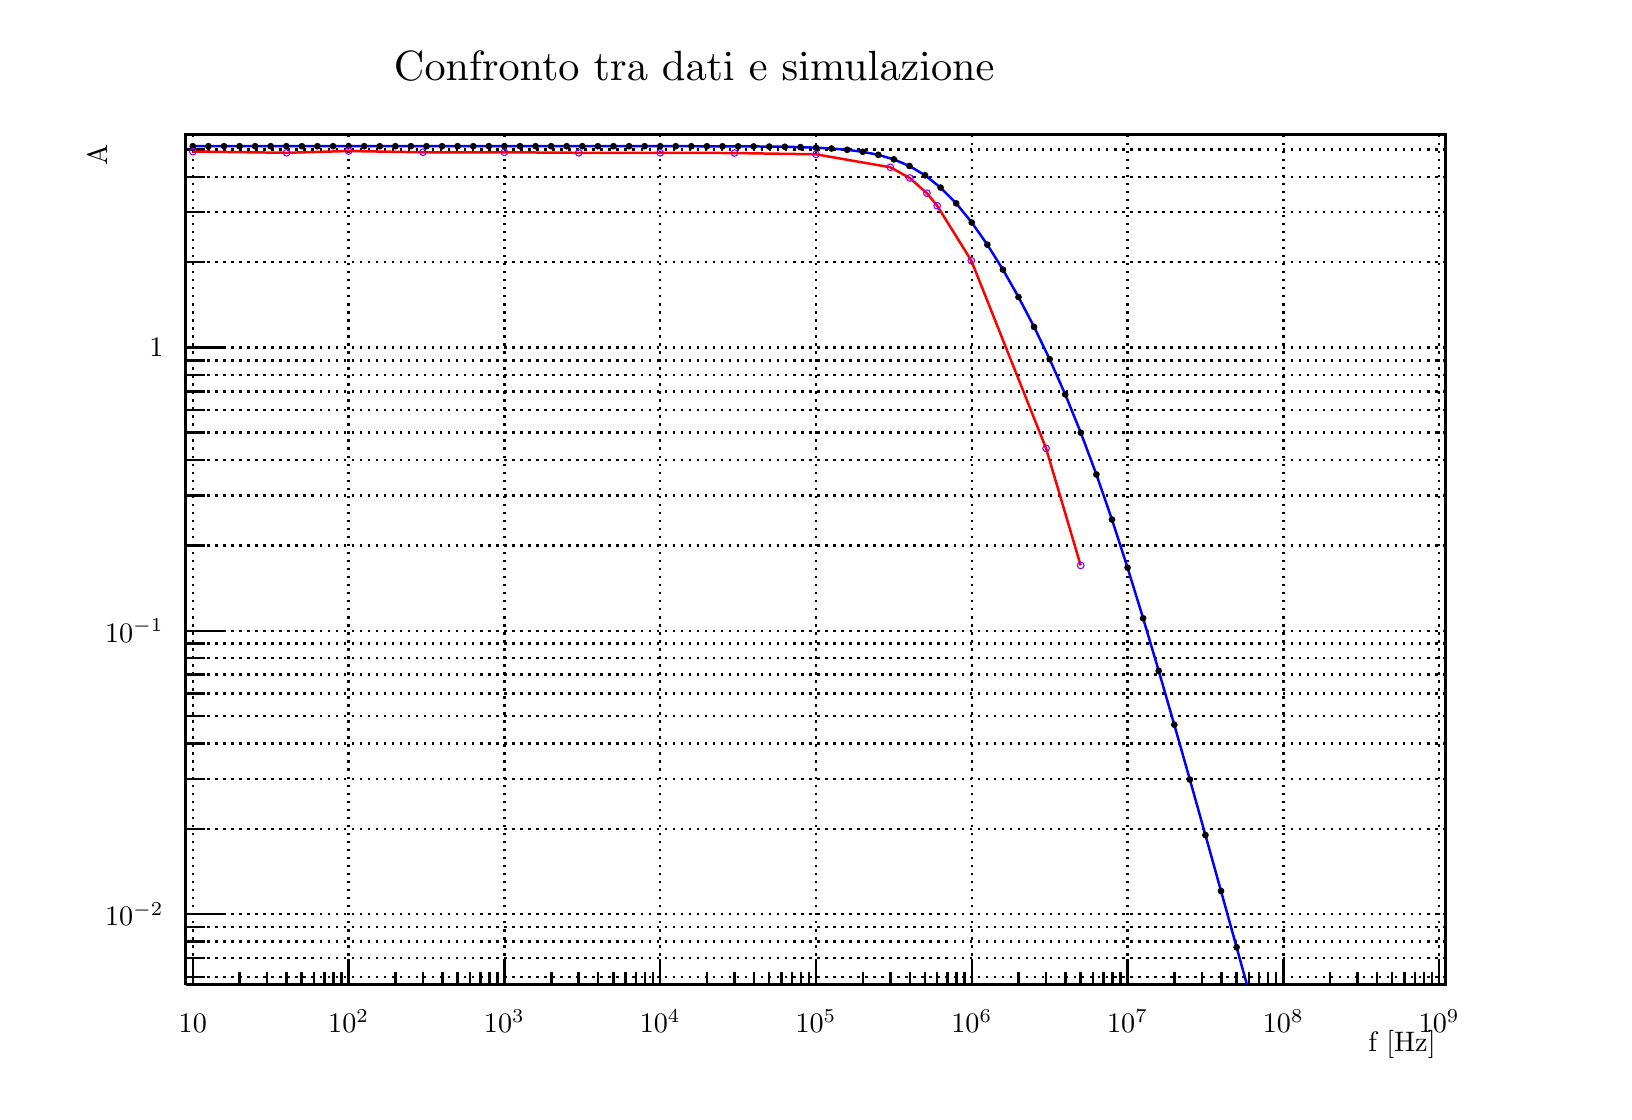
\begin{tikzpicture}
\pgfdeclareplotmark{cross} {
\pgfpathmoveto{\pgfpoint{-0.3\pgfplotmarksize}{\pgfplotmarksize}}
\pgfpathlineto{\pgfpoint{+0.3\pgfplotmarksize}{\pgfplotmarksize}}
\pgfpathlineto{\pgfpoint{+0.3\pgfplotmarksize}{0.3\pgfplotmarksize}}
\pgfpathlineto{\pgfpoint{+1\pgfplotmarksize}{0.3\pgfplotmarksize}}
\pgfpathlineto{\pgfpoint{+1\pgfplotmarksize}{-0.3\pgfplotmarksize}}
\pgfpathlineto{\pgfpoint{+0.3\pgfplotmarksize}{-0.3\pgfplotmarksize}}
\pgfpathlineto{\pgfpoint{+0.3\pgfplotmarksize}{-1.\pgfplotmarksize}}
\pgfpathlineto{\pgfpoint{-0.3\pgfplotmarksize}{-1.\pgfplotmarksize}}
\pgfpathlineto{\pgfpoint{-0.3\pgfplotmarksize}{-0.3\pgfplotmarksize}}
\pgfpathlineto{\pgfpoint{-1.\pgfplotmarksize}{-0.3\pgfplotmarksize}}
\pgfpathlineto{\pgfpoint{-1.\pgfplotmarksize}{0.3\pgfplotmarksize}}
\pgfpathlineto{\pgfpoint{-0.3\pgfplotmarksize}{0.3\pgfplotmarksize}}
\pgfpathclose
\pgfusepathqstroke
}
\pgfdeclareplotmark{cross*} {
\pgfpathmoveto{\pgfpoint{-0.3\pgfplotmarksize}{\pgfplotmarksize}}
\pgfpathlineto{\pgfpoint{+0.3\pgfplotmarksize}{\pgfplotmarksize}}
\pgfpathlineto{\pgfpoint{+0.3\pgfplotmarksize}{0.3\pgfplotmarksize}}
\pgfpathlineto{\pgfpoint{+1\pgfplotmarksize}{0.3\pgfplotmarksize}}
\pgfpathlineto{\pgfpoint{+1\pgfplotmarksize}{-0.3\pgfplotmarksize}}
\pgfpathlineto{\pgfpoint{+0.3\pgfplotmarksize}{-0.3\pgfplotmarksize}}
\pgfpathlineto{\pgfpoint{+0.3\pgfplotmarksize}{-1.\pgfplotmarksize}}
\pgfpathlineto{\pgfpoint{-0.3\pgfplotmarksize}{-1.\pgfplotmarksize}}
\pgfpathlineto{\pgfpoint{-0.3\pgfplotmarksize}{-0.3\pgfplotmarksize}}
\pgfpathlineto{\pgfpoint{-1.\pgfplotmarksize}{-0.3\pgfplotmarksize}}
\pgfpathlineto{\pgfpoint{-1.\pgfplotmarksize}{0.3\pgfplotmarksize}}
\pgfpathlineto{\pgfpoint{-0.3\pgfplotmarksize}{0.3\pgfplotmarksize}}
\pgfpathclose
\pgfusepathqfillstroke
}
\pgfdeclareplotmark{newstar} {
\pgfpathmoveto{\pgfqpoint{0pt}{\pgfplotmarksize}}
\pgfpathlineto{\pgfqpointpolar{44}{0.5\pgfplotmarksize}}
\pgfpathlineto{\pgfqpointpolar{18}{\pgfplotmarksize}}
\pgfpathlineto{\pgfqpointpolar{-20}{0.5\pgfplotmarksize}}
\pgfpathlineto{\pgfqpointpolar{-54}{\pgfplotmarksize}}
\pgfpathlineto{\pgfqpointpolar{-90}{0.5\pgfplotmarksize}}
\pgfpathlineto{\pgfqpointpolar{234}{\pgfplotmarksize}}
\pgfpathlineto{\pgfqpointpolar{198}{0.5\pgfplotmarksize}}
\pgfpathlineto{\pgfqpointpolar{162}{\pgfplotmarksize}}
\pgfpathlineto{\pgfqpointpolar{134}{0.5\pgfplotmarksize}}
\pgfpathclose
\pgfusepathqstroke
}
\pgfdeclareplotmark{newstar*} {
\pgfpathmoveto{\pgfqpoint{0pt}{\pgfplotmarksize}}
\pgfpathlineto{\pgfqpointpolar{44}{0.5\pgfplotmarksize}}
\pgfpathlineto{\pgfqpointpolar{18}{\pgfplotmarksize}}
\pgfpathlineto{\pgfqpointpolar{-20}{0.5\pgfplotmarksize}}
\pgfpathlineto{\pgfqpointpolar{-54}{\pgfplotmarksize}}
\pgfpathlineto{\pgfqpointpolar{-90}{0.5\pgfplotmarksize}}
\pgfpathlineto{\pgfqpointpolar{234}{\pgfplotmarksize}}
\pgfpathlineto{\pgfqpointpolar{198}{0.5\pgfplotmarksize}}
\pgfpathlineto{\pgfqpointpolar{162}{\pgfplotmarksize}}
\pgfpathlineto{\pgfqpointpolar{134}{0.5\pgfplotmarksize}}
\pgfpathclose
\pgfusepathqfillstroke
}
\definecolor{c}{rgb}{1,1,1};
\draw [color=c, fill=c] (0,0) rectangle (20,13.4957);
\draw [color=c, fill=c] (2,1.34957) rectangle (18,12.1461);
\definecolor{c}{rgb}{0,0,0};
\draw [c,line width=0.9] (2,1.34957) -- (2,12.1461) -- (18,12.1461) -- (18,1.34957) -- (2,1.34957);
\definecolor{c}{rgb}{1,1,1};
\draw [color=c, fill=c] (2,1.34957) rectangle (18,12.1461);
\definecolor{c}{rgb}{0,0,0};
\draw [c,line width=0.9] (2,1.34957) -- (2,12.1461) -- (18,12.1461) -- (18,1.34957) -- (2,1.34957);
\draw [c,line width=0.9] (2,1.34957) -- (18,1.34957);
\draw [c,dotted,line width=0.9] (2.09053,12.1461) -- (2.09053,1.34957);
\draw [c,dotted,line width=0.9] (4.06897,12.1461) -- (4.06897,1.34957);
\draw [c,dotted,line width=0.9] (6.04742,12.1461) -- (6.04742,1.34957);
\draw [c,dotted,line width=0.9] (8.02587,12.1461) -- (8.02587,1.34957);
\draw [c,dotted,line width=0.9] (10.0043,12.1461) -- (10.0043,1.34957);
\draw [c,dotted,line width=0.9] (11.9828,12.1461) -- (11.9828,1.34957);
\draw [c,dotted,line width=0.9] (13.9612,12.1461) -- (13.9612,1.34957);
\draw [c,dotted,line width=0.9] (15.9397,12.1461) -- (15.9397,1.34957);
\draw [c,dotted,line width=0.9] (17.9181,12.1461) -- (17.9181,1.34957);
\draw [c,line width=0.9] (2,1.34957) -- (2,12.1461);
\draw [c,dotted,line width=0.9] (18,1.44637) -- (2,1.44637);
\draw [c,dotted,line width=0.9] (18,1.68731) -- (2,1.68731);
\draw [c,dotted,line width=0.9] (18,1.89601) -- (2,1.89601);
\draw [c,dotted,line width=0.9] (18,2.0801) -- (2,2.0801);
\draw [c,dotted,line width=0.9] (18,2.24478) -- (2,2.24478);
\draw [c,dotted,line width=0.9] (18,3.32814) -- (2,3.32814);
\draw [c,dotted,line width=0.9] (18,3.96186) -- (2,3.96186);
\draw [c,dotted,line width=0.9] (18,4.4115) -- (2,4.4115);
\draw [c,dotted,line width=0.9] (18,4.76027) -- (2,4.76027);
\draw [c,dotted,line width=0.9] (18,5.04523) -- (2,5.04523);
\draw [c,dotted,line width=0.9] (18,5.28616) -- (2,5.28616);
\draw [c,dotted,line width=0.9] (18,5.49486) -- (2,5.49486);
\draw [c,dotted,line width=0.9] (18,5.67895) -- (2,5.67895);
\draw [c,dotted,line width=0.9] (18,5.84363) -- (2,5.84363);
\draw [c,dotted,line width=0.9] (18,6.92699) -- (2,6.92699);
\draw [c,dotted,line width=0.9] (18,7.56072) -- (2,7.56072);
\draw [c,dotted,line width=0.9] (18,8.01035) -- (2,8.01035);
\draw [c,dotted,line width=0.9] (18,8.35912) -- (2,8.35912);
\draw [c,dotted,line width=0.9] (18,8.64408) -- (2,8.64408);
\draw [c,dotted,line width=0.9] (18,8.88501) -- (2,8.88501);
\draw [c,dotted,line width=0.9] (18,9.09372) -- (2,9.09372);
\draw [c,dotted,line width=0.9] (18,9.27781) -- (2,9.27781);
\draw [c,dotted,line width=0.9] (18,9.44248) -- (2,9.44248);
\draw [c,dotted,line width=0.9] (18,10.5258) -- (2,10.5258);
\draw [c,dotted,line width=0.9] (18,11.1596) -- (2,11.1596);
\draw [c,dotted,line width=0.9] (18,11.6092) -- (2,11.6092);
\draw [c,dotted,line width=0.9] (18,11.958) -- (2,11.958);
\draw [c,line width=0.9] (2,1.34957) -- (18,1.34957);
\draw [anchor= east] (18,0.593811) node[scale=1.01821, color=c, rotate=0]{f [Hz]};
\draw [c,line width=0.9] (2.09053,1.67347) -- (2.09053,1.34957);
\draw [anchor=base] (2.09053,0.73889) node[scale=1.01821, color=c, rotate=0]{10};
\draw [c,line width=0.9] (2.6861,1.51152) -- (2.6861,1.34957);
\draw [c,line width=0.9] (3.03449,1.51152) -- (3.03449,1.34957);
\draw [c,line width=0.9] (3.28167,1.51152) -- (3.28167,1.34957);
\draw [c,line width=0.9] (3.4734,1.51152) -- (3.4734,1.34957);
\draw [c,line width=0.9] (3.63006,1.51152) -- (3.63006,1.34957);
\draw [c,line width=0.9] (3.76251,1.51152) -- (3.76251,1.34957);
\draw [c,line width=0.9] (3.87724,1.51152) -- (3.87724,1.34957);
\draw [c,line width=0.9] (3.97845,1.51152) -- (3.97845,1.34957);
\draw [c,line width=0.9] (4.06897,1.67347) -- (4.06897,1.34957);
\draw [anchor=base] (4.06897,0.73889) node[scale=1.01821, color=c, rotate=0]{$10^{2}$};
\draw [c,line width=0.9] (4.66455,1.51152) -- (4.66455,1.34957);
\draw [c,line width=0.9] (5.01293,1.51152) -- (5.01293,1.34957);
\draw [c,line width=0.9] (5.26012,1.51152) -- (5.26012,1.34957);
\draw [c,line width=0.9] (5.45185,1.51152) -- (5.45185,1.34957);
\draw [c,line width=0.9] (5.60851,1.51152) -- (5.60851,1.34957);
\draw [c,line width=0.9] (5.74096,1.51152) -- (5.74096,1.34957);
\draw [c,line width=0.9] (5.85569,1.51152) -- (5.85569,1.34957);
\draw [c,line width=0.9] (5.95689,1.51152) -- (5.95689,1.34957);
\draw [c,line width=0.9] (6.04742,1.67347) -- (6.04742,1.34957);
\draw [anchor=base] (6.04742,0.73889) node[scale=1.01821, color=c, rotate=0]{$10^{3}$};
\draw [c,line width=0.9] (6.64299,1.51152) -- (6.64299,1.34957);
\draw [c,line width=0.9] (6.99138,1.51152) -- (6.99138,1.34957);
\draw [c,line width=0.9] (7.23857,1.51152) -- (7.23857,1.34957);
\draw [c,line width=0.9] (7.4303,1.51152) -- (7.4303,1.34957);
\draw [c,line width=0.9] (7.58695,1.51152) -- (7.58695,1.34957);
\draw [c,line width=0.9] (7.7194,1.51152) -- (7.7194,1.34957);
\draw [c,line width=0.9] (7.83414,1.51152) -- (7.83414,1.34957);
\draw [c,line width=0.9] (7.93534,1.51152) -- (7.93534,1.34957);
\draw [c,line width=0.9] (8.02587,1.67347) -- (8.02587,1.34957);
\draw [anchor=base] (8.02587,0.73889) node[scale=1.01821, color=c, rotate=0]{$10^{4}$};
\draw [c,line width=0.9] (8.62144,1.51152) -- (8.62144,1.34957);
\draw [c,line width=0.9] (8.96983,1.51152) -- (8.96983,1.34957);
\draw [c,line width=0.9] (9.21701,1.51152) -- (9.21701,1.34957);
\draw [c,line width=0.9] (9.40874,1.51152) -- (9.40874,1.34957);
\draw [c,line width=0.9] (9.5654,1.51152) -- (9.5654,1.34957);
\draw [c,line width=0.9] (9.69785,1.51152) -- (9.69785,1.34957);
\draw [c,line width=0.9] (9.81259,1.51152) -- (9.81259,1.34957);
\draw [c,line width=0.9] (9.91379,1.51152) -- (9.91379,1.34957);
\draw [c,line width=0.9] (10.0043,1.67347) -- (10.0043,1.34957);
\draw [anchor=base] (10.0043,0.73889) node[scale=1.01821, color=c, rotate=0]{$10^{5}$};
\draw [c,line width=0.9] (10.5999,1.51152) -- (10.5999,1.34957);
\draw [c,line width=0.9] (10.9483,1.51152) -- (10.9483,1.34957);
\draw [c,line width=0.9] (11.1955,1.51152) -- (11.1955,1.34957);
\draw [c,line width=0.9] (11.3872,1.51152) -- (11.3872,1.34957);
\draw [c,line width=0.9] (11.5438,1.51152) -- (11.5438,1.34957);
\draw [c,line width=0.9] (11.6763,1.51152) -- (11.6763,1.34957);
\draw [c,line width=0.9] (11.791,1.51152) -- (11.791,1.34957);
\draw [c,line width=0.9] (11.8922,1.51152) -- (11.8922,1.34957);
\draw [c,line width=0.9] (11.9828,1.67347) -- (11.9828,1.34957);
\draw [anchor=base] (11.9828,0.73889) node[scale=1.01821, color=c, rotate=0]{$10^{6}$};
\draw [c,line width=0.9] (12.5783,1.51152) -- (12.5783,1.34957);
\draw [c,line width=0.9] (12.9267,1.51152) -- (12.9267,1.34957);
\draw [c,line width=0.9] (13.1739,1.51152) -- (13.1739,1.34957);
\draw [c,line width=0.9] (13.3656,1.51152) -- (13.3656,1.34957);
\draw [c,line width=0.9] (13.5223,1.51152) -- (13.5223,1.34957);
\draw [c,line width=0.9] (13.6547,1.51152) -- (13.6547,1.34957);
\draw [c,line width=0.9] (13.7695,1.51152) -- (13.7695,1.34957);
\draw [c,line width=0.9] (13.8707,1.51152) -- (13.8707,1.34957);
\draw [c,line width=0.9] (13.9612,1.67347) -- (13.9612,1.34957);
\draw [anchor=base] (13.9612,0.73889) node[scale=1.01821, color=c, rotate=0]{$10^{7}$};
\draw [c,line width=0.9] (14.5568,1.51152) -- (14.5568,1.34957);
\draw [c,line width=0.9] (14.9052,1.51152) -- (14.9052,1.34957);
\draw [c,line width=0.9] (15.1524,1.51152) -- (15.1524,1.34957);
\draw [c,line width=0.9] (15.3441,1.51152) -- (15.3441,1.34957);
\draw [c,line width=0.9] (15.5007,1.51152) -- (15.5007,1.34957);
\draw [c,line width=0.9] (15.6332,1.51152) -- (15.6332,1.34957);
\draw [c,line width=0.9] (15.7479,1.51152) -- (15.7479,1.34957);
\draw [c,line width=0.9] (15.8491,1.51152) -- (15.8491,1.34957);
\draw [c,line width=0.9] (15.9397,1.67347) -- (15.9397,1.34957);
\draw [anchor=base] (15.9397,0.73889) node[scale=1.01821, color=c, rotate=0]{$10^{8}$};
\draw [c,line width=0.9] (16.5352,1.51152) -- (16.5352,1.34957);
\draw [c,line width=0.9] (16.8836,1.51152) -- (16.8836,1.34957);
\draw [c,line width=0.9] (17.1308,1.51152) -- (17.1308,1.34957);
\draw [c,line width=0.9] (17.3225,1.51152) -- (17.3225,1.34957);
\draw [c,line width=0.9] (17.4792,1.51152) -- (17.4792,1.34957);
\draw [c,line width=0.9] (17.6116,1.51152) -- (17.6116,1.34957);
\draw [c,line width=0.9] (17.7264,1.51152) -- (17.7264,1.34957);
\draw [c,line width=0.9] (17.8276,1.51152) -- (17.8276,1.34957);
\draw [c,line width=0.9] (17.9181,1.67347) -- (17.9181,1.34957);
\draw [anchor=base] (17.9181,0.73889) node[scale=1.01821, color=c, rotate=0]{$10^{9}$};
\draw [c,line width=0.9] (2,1.34957) -- (2,12.1461);
\draw [anchor= east] (0.88,12.1461) node[scale=1.01821, color=c, rotate=90]{A};
\draw [c,line width=0.9] (2.24,1.44637) -- (2,1.44637);
\draw [c,line width=0.9] (2.24,1.68731) -- (2,1.68731);
\draw [c,line width=0.9] (2.24,1.89601) -- (2,1.89601);
\draw [c,line width=0.9] (2.24,2.0801) -- (2,2.0801);
\draw [c,line width=0.9] (2.48,2.24478) -- (2,2.24478);
\draw [anchor= east] (1.844,2.24478) node[scale=1.01821, color=c, rotate=0]{$10^{-2}$};
\draw [c,line width=0.9] (2.24,3.32814) -- (2,3.32814);
\draw [c,line width=0.9] (2.24,3.96186) -- (2,3.96186);
\draw [c,line width=0.9] (2.24,4.4115) -- (2,4.4115);
\draw [c,line width=0.9] (2.24,4.76027) -- (2,4.76027);
\draw [c,line width=0.9] (2.24,5.04523) -- (2,5.04523);
\draw [c,line width=0.9] (2.24,5.28616) -- (2,5.28616);
\draw [c,line width=0.9] (2.24,5.49486) -- (2,5.49486);
\draw [c,line width=0.9] (2.24,5.67895) -- (2,5.67895);
\draw [c,line width=0.9] (2.48,5.84363) -- (2,5.84363);
\draw [anchor= east] (1.844,5.84363) node[scale=1.01821, color=c, rotate=0]{$10^{-1}$};
\draw [c,line width=0.9] (2.24,6.92699) -- (2,6.92699);
\draw [c,line width=0.9] (2.24,7.56072) -- (2,7.56072);
\draw [c,line width=0.9] (2.24,8.01035) -- (2,8.01035);
\draw [c,line width=0.9] (2.24,8.35912) -- (2,8.35912);
\draw [c,line width=0.9] (2.24,8.64408) -- (2,8.64408);
\draw [c,line width=0.9] (2.24,8.88501) -- (2,8.88501);
\draw [c,line width=0.9] (2.24,9.09372) -- (2,9.09372);
\draw [c,line width=0.9] (2.24,9.27781) -- (2,9.27781);
\draw [c,line width=0.9] (2.48,9.44248) -- (2,9.44248);
\draw [anchor= east] (1.844,9.44248) node[scale=1.01821, color=c, rotate=0]{1};
\draw [c,line width=0.9] (2.24,10.5258) -- (2,10.5258);
\draw [c,line width=0.9] (2.24,11.1596) -- (2,11.1596);
\draw [c,line width=0.9] (2.24,11.6092) -- (2,11.6092);
\draw [c,line width=0.9] (2.24,11.958) -- (2,11.958);
\definecolor{c}{rgb}{0,0,1};
\draw [c,line width=0.9] (2.09053,11.9972) -- (2.28837,11.9972) -- (2.48622,11.9972) -- (2.68406,11.9972) -- (2.88191,11.9972) -- (3.07975,11.9972) -- (3.2776,11.9972) -- (3.47544,11.9972) -- (3.67329,11.9972) -- (3.87113,11.9972) --
 (4.06898,11.9972) -- (4.26682,11.9972) -- (4.46467,11.9972) -- (4.66251,11.9972) -- (4.86035,11.9972) -- (5.0582,11.9972) -- (5.25604,11.9972) -- (5.45389,11.9972) -- (5.65173,11.9972) -- (5.84958,11.9972) -- (6.04742,11.9972) -- (6.24527,11.9972)
 -- (6.44311,11.9972) -- (6.64096,11.9972) -- (6.8388,11.9972) -- (7.03665,11.9971) -- (7.23449,11.9971) -- (7.43234,11.9971) -- (7.63018,11.9971) -- (7.82803,11.997) -- (8.02587,11.997) -- (8.22371,11.9969) -- (8.42156,11.9967) -- (8.6194,11.9964)
 -- (8.81725,11.996) -- (9.01509,11.9953) -- (9.21294,11.9942) -- (9.41078,11.9925) -- (9.60863,11.9898) -- (9.80647,11.9855) -- (10.0043,11.9788) -- (10.2022,11.9682) -- (10.4,11.9517) -- (10.5979,11.9263) -- (10.7957,11.8875) -- (10.9935,11.8297)
 -- (11.1914,11.7458) -- (11.3892,11.6285) -- (11.5871,11.4714) -- (11.7849,11.2714) -- (11.9828,11.0288) -- (12.1806,10.7468) -- (12.3785,10.43) -- (12.5763,10.0817) -- (12.7741,9.703) -- (12.972,9.29213) -- (13.1698,8.84535) -- (13.3677,8.35833) --
 (13.5655,7.82829) -- (13.7634,7.25572) -- (13.9612,6.64474) -- (14.1591,6.00201) -- (14.3569,5.33493) -- (14.5547,4.65027) -- (14.7526,3.95347) -- (14.9504,3.24855) -- (15.1483,2.53828) -- (15.3461,1.82457) -- (15.4774,1.34957);
\definecolor{c}{rgb}{0,0,0};
\foreach \P in {(2.09053,11.9972), (2.28837,11.9972), (2.48622,11.9972), (2.68406,11.9972), (2.88191,11.9972), (3.07975,11.9972), (3.2776,11.9972), (3.47544,11.9972), (3.67329,11.9972), (3.87113,11.9972), (4.06898,11.9972), (4.26682,11.9972),
 (4.46467,11.9972), (4.66251,11.9972), (4.86035,11.9972), (5.0582,11.9972), (5.25604,11.9972), (5.45389,11.9972), (5.65173,11.9972), (5.84958,11.9972), (6.04742,11.9972), (6.24527,11.9972), (6.44311,11.9972), (6.64096,11.9972), (6.8388,11.9972),
 (7.03665,11.9971), (7.23449,11.9971), (7.43234,11.9971), (7.63018,11.9971), (7.82803,11.997), (8.02587,11.997), (8.22371,11.9969), (8.42156,11.9967), (8.6194,11.9964), (8.81725,11.996), (9.01509,11.9953), (9.21294,11.9942), (9.41078,11.9925),
 (9.60863,11.9898), (9.80647,11.9855), (10.0043,11.9788), (10.2022,11.9682), (10.4,11.9517), (10.5979,11.9263), (10.7957,11.8875), (10.9935,11.8297), (11.1914,11.7458), (11.3892,11.6285), (11.5871,11.4714), (11.7849,11.2714), (11.9828,11.0288),
 (12.1806,10.7468), (12.3785,10.43), (12.5763,10.0817), (12.7741,9.703), (12.972,9.29213), (13.1698,8.84535), (13.3677,8.35833), (13.5655,7.82829), (13.7634,7.25572), (13.9612,6.64474), (14.1591,6.00201), (14.3569,5.33493), (14.5547,4.65027),
 (14.7526,3.95347), (14.9504,3.24855), (15.1483,2.53828), (15.3461,1.82457)}{\draw[mark options={color=c,fill=c},mark size=2.402402pt,mark=*,mark size=1pt] plot coordinates {\P};}
\draw (8.45788,13.0156) node[scale=1.52731, color=c, rotate=0]{Confronto tra dati e simulazione};
\definecolor{c}{rgb}{1,0,0};
\draw [c,line width=0.9] (2.09053,11.9296) -- (3.28167,11.9136) -- (4.06898,11.9359) -- (5.01294,11.92) -- (6.04742,11.92) -- (6.99138,11.9136) -- (8.02587,11.9136) -- (8.96983,11.9104) -- (10.0043,11.8942) -- (10.9483,11.7295) -- (11.1955,11.5935)
 -- (11.4126,11.4005) -- (11.5438,11.2408) -- (11.9771,10.5444) -- (12.9267,8.15932) -- (13.3656,6.67298);
\definecolor{c}{rgb}{0.573333,0,1};
\foreach \P in {(2.09053,11.9296), (3.28167,11.9136), (4.06898,11.9359), (5.01294,11.92), (6.04742,11.92), (6.99138,11.9136), (8.02587,11.9136), (8.96983,11.9104), (10.0043,11.8942), (10.9483,11.7295), (11.1955,11.5935), (11.4126,11.4005),
 (11.5438,11.2408), (11.9771,10.5444), (12.9267,8.15932), (13.3656,6.67298)}{\draw[mark options={color=c,fill=c},mark size=1.201201pt,mark=o] plot coordinates {\P};}
\end{tikzpicture}

 }%
 \caption{Risposta in frequenza con Spice confrontata coi dati sperimentali (A=5)} 
 \label{gr:sim_a5.tex} 
\end{grafico}

\begin{grafico}
 \centering
 \resizebox{\textwidth}{!}{%
 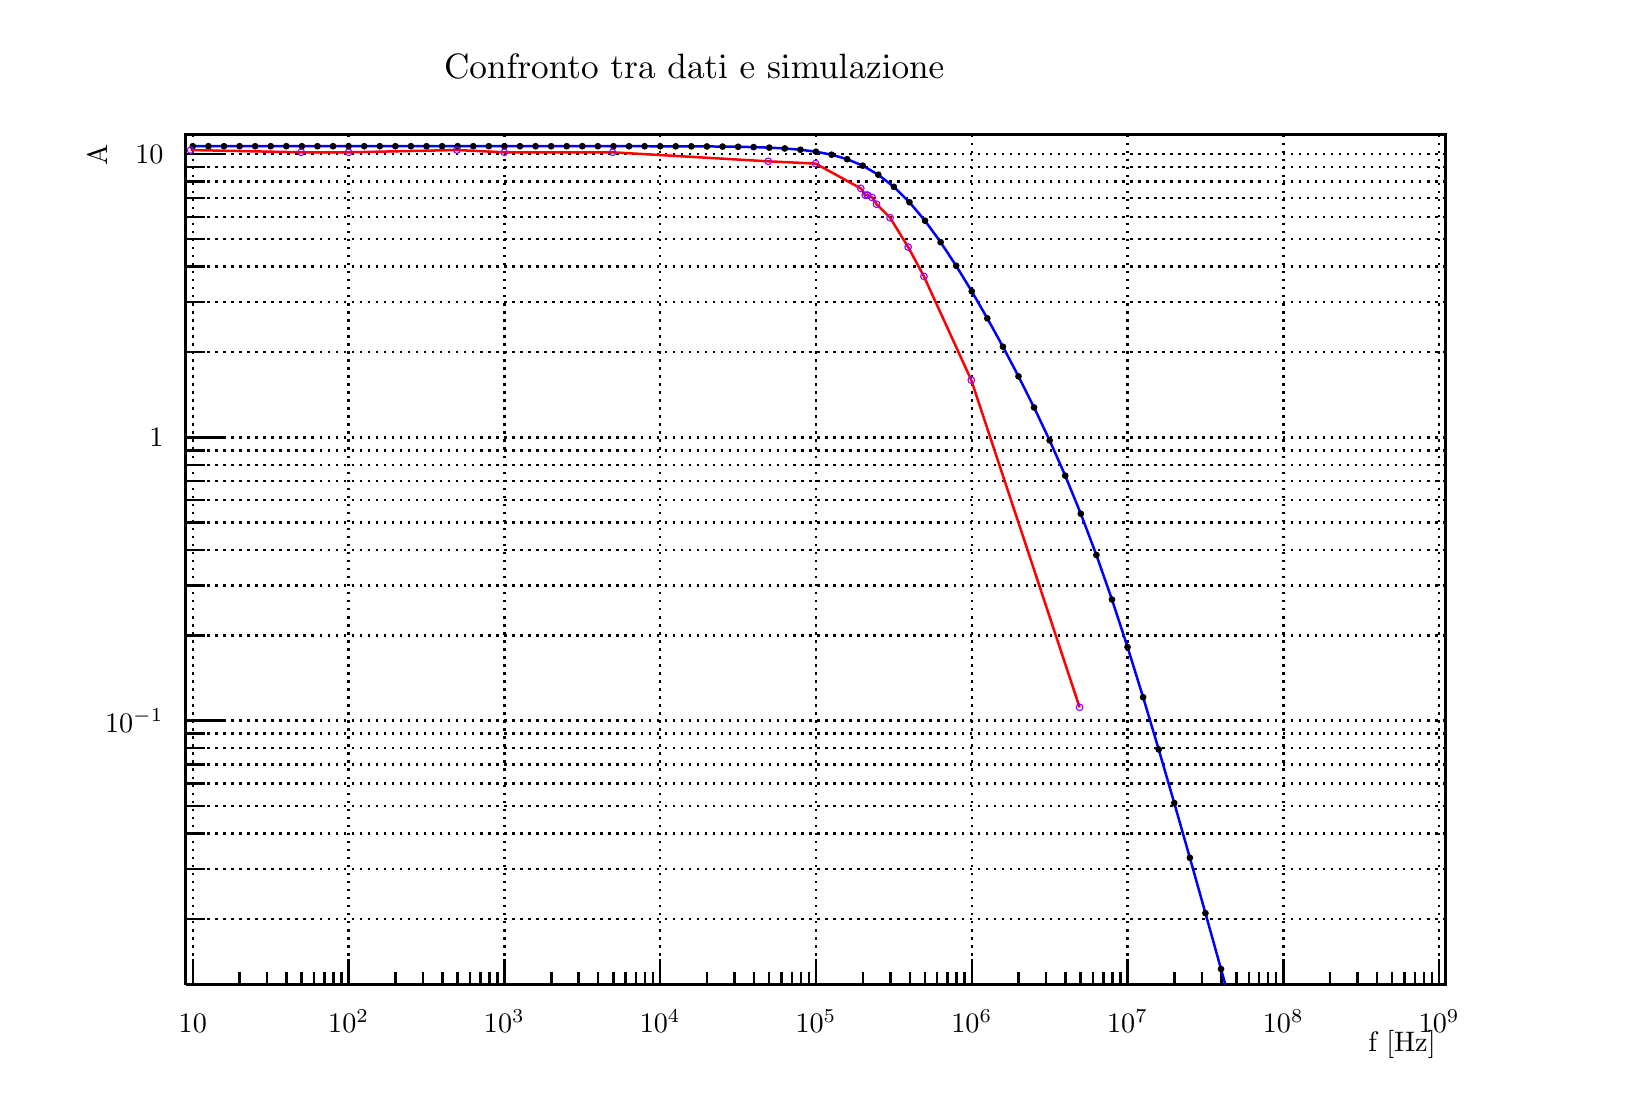
\begin{tikzpicture}
\pgfdeclareplotmark{cross} {
\pgfpathmoveto{\pgfpoint{-0.3\pgfplotmarksize}{\pgfplotmarksize}}
\pgfpathlineto{\pgfpoint{+0.3\pgfplotmarksize}{\pgfplotmarksize}}
\pgfpathlineto{\pgfpoint{+0.3\pgfplotmarksize}{0.3\pgfplotmarksize}}
\pgfpathlineto{\pgfpoint{+1\pgfplotmarksize}{0.3\pgfplotmarksize}}
\pgfpathlineto{\pgfpoint{+1\pgfplotmarksize}{-0.3\pgfplotmarksize}}
\pgfpathlineto{\pgfpoint{+0.3\pgfplotmarksize}{-0.3\pgfplotmarksize}}
\pgfpathlineto{\pgfpoint{+0.3\pgfplotmarksize}{-1.\pgfplotmarksize}}
\pgfpathlineto{\pgfpoint{-0.3\pgfplotmarksize}{-1.\pgfplotmarksize}}
\pgfpathlineto{\pgfpoint{-0.3\pgfplotmarksize}{-0.3\pgfplotmarksize}}
\pgfpathlineto{\pgfpoint{-1.\pgfplotmarksize}{-0.3\pgfplotmarksize}}
\pgfpathlineto{\pgfpoint{-1.\pgfplotmarksize}{0.3\pgfplotmarksize}}
\pgfpathlineto{\pgfpoint{-0.3\pgfplotmarksize}{0.3\pgfplotmarksize}}
\pgfpathclose
\pgfusepathqstroke
}
\pgfdeclareplotmark{cross*} {
\pgfpathmoveto{\pgfpoint{-0.3\pgfplotmarksize}{\pgfplotmarksize}}
\pgfpathlineto{\pgfpoint{+0.3\pgfplotmarksize}{\pgfplotmarksize}}
\pgfpathlineto{\pgfpoint{+0.3\pgfplotmarksize}{0.3\pgfplotmarksize}}
\pgfpathlineto{\pgfpoint{+1\pgfplotmarksize}{0.3\pgfplotmarksize}}
\pgfpathlineto{\pgfpoint{+1\pgfplotmarksize}{-0.3\pgfplotmarksize}}
\pgfpathlineto{\pgfpoint{+0.3\pgfplotmarksize}{-0.3\pgfplotmarksize}}
\pgfpathlineto{\pgfpoint{+0.3\pgfplotmarksize}{-1.\pgfplotmarksize}}
\pgfpathlineto{\pgfpoint{-0.3\pgfplotmarksize}{-1.\pgfplotmarksize}}
\pgfpathlineto{\pgfpoint{-0.3\pgfplotmarksize}{-0.3\pgfplotmarksize}}
\pgfpathlineto{\pgfpoint{-1.\pgfplotmarksize}{-0.3\pgfplotmarksize}}
\pgfpathlineto{\pgfpoint{-1.\pgfplotmarksize}{0.3\pgfplotmarksize}}
\pgfpathlineto{\pgfpoint{-0.3\pgfplotmarksize}{0.3\pgfplotmarksize}}
\pgfpathclose
\pgfusepathqfillstroke
}
\pgfdeclareplotmark{newstar} {
\pgfpathmoveto{\pgfqpoint{0pt}{\pgfplotmarksize}}
\pgfpathlineto{\pgfqpointpolar{44}{0.5\pgfplotmarksize}}
\pgfpathlineto{\pgfqpointpolar{18}{\pgfplotmarksize}}
\pgfpathlineto{\pgfqpointpolar{-20}{0.5\pgfplotmarksize}}
\pgfpathlineto{\pgfqpointpolar{-54}{\pgfplotmarksize}}
\pgfpathlineto{\pgfqpointpolar{-90}{0.5\pgfplotmarksize}}
\pgfpathlineto{\pgfqpointpolar{234}{\pgfplotmarksize}}
\pgfpathlineto{\pgfqpointpolar{198}{0.5\pgfplotmarksize}}
\pgfpathlineto{\pgfqpointpolar{162}{\pgfplotmarksize}}
\pgfpathlineto{\pgfqpointpolar{134}{0.5\pgfplotmarksize}}
\pgfpathclose
\pgfusepathqstroke
}
\pgfdeclareplotmark{newstar*} {
\pgfpathmoveto{\pgfqpoint{0pt}{\pgfplotmarksize}}
\pgfpathlineto{\pgfqpointpolar{44}{0.5\pgfplotmarksize}}
\pgfpathlineto{\pgfqpointpolar{18}{\pgfplotmarksize}}
\pgfpathlineto{\pgfqpointpolar{-20}{0.5\pgfplotmarksize}}
\pgfpathlineto{\pgfqpointpolar{-54}{\pgfplotmarksize}}
\pgfpathlineto{\pgfqpointpolar{-90}{0.5\pgfplotmarksize}}
\pgfpathlineto{\pgfqpointpolar{234}{\pgfplotmarksize}}
\pgfpathlineto{\pgfqpointpolar{198}{0.5\pgfplotmarksize}}
\pgfpathlineto{\pgfqpointpolar{162}{\pgfplotmarksize}}
\pgfpathlineto{\pgfqpointpolar{134}{0.5\pgfplotmarksize}}
\pgfpathclose
\pgfusepathqfillstroke
}
\definecolor{c}{rgb}{1,1,1};
\draw [color=c, fill=c] (0,0) rectangle (20,13.4957);
\draw [color=c, fill=c] (2,1.34957) rectangle (18,12.1461);
\definecolor{c}{rgb}{0,0,0};
\draw [c,line width=0.9] (2,1.34957) -- (2,12.1461) -- (18,12.1461) -- (18,1.34957) -- (2,1.34957);
\definecolor{c}{rgb}{1,1,1};
\draw [color=c, fill=c] (2,1.34957) rectangle (18,12.1461);
\definecolor{c}{rgb}{0,0,0};
\draw [c,line width=0.9] (2,1.34957) -- (2,12.1461) -- (18,12.1461) -- (18,1.34957) -- (2,1.34957);
\draw [c,line width=0.9] (2,1.34957) -- (18,1.34957);
\draw [c,dotted,line width=0.9] (2.09053,12.1461) -- (2.09053,1.34957);
\draw [c,dotted,line width=0.9] (4.06897,12.1461) -- (4.06897,1.34957);
\draw [c,dotted,line width=0.9] (6.04742,12.1461) -- (6.04742,1.34957);
\draw [c,dotted,line width=0.9] (8.02587,12.1461) -- (8.02587,1.34957);
\draw [c,dotted,line width=0.9] (10.0043,12.1461) -- (10.0043,1.34957);
\draw [c,dotted,line width=0.9] (11.9828,12.1461) -- (11.9828,1.34957);
\draw [c,dotted,line width=0.9] (13.9612,12.1461) -- (13.9612,1.34957);
\draw [c,dotted,line width=0.9] (15.9397,12.1461) -- (15.9397,1.34957);
\draw [c,dotted,line width=0.9] (17.9181,12.1461) -- (17.9181,1.34957);
\draw [c,line width=0.9] (2,1.34957) -- (2,12.1461);
\draw [c,dotted,line width=0.9] (18,2.18589) -- (2,2.18589);
\draw [c,dotted,line width=0.9] (18,2.81962) -- (2,2.81962);
\draw [c,dotted,line width=0.9] (18,3.26926) -- (2,3.26926);
\draw [c,dotted,line width=0.9] (18,3.61802) -- (2,3.61802);
\draw [c,dotted,line width=0.9] (18,3.90298) -- (2,3.90298);
\draw [c,dotted,line width=0.9] (18,4.14391) -- (2,4.14391);
\draw [c,dotted,line width=0.9] (18,4.35262) -- (2,4.35262);
\draw [c,dotted,line width=0.9] (18,4.53671) -- (2,4.53671);
\draw [c,dotted,line width=0.9] (18,4.70138) -- (2,4.70138);
\draw [c,dotted,line width=0.9] (18,5.78475) -- (2,5.78475);
\draw [c,dotted,line width=0.9] (18,6.41847) -- (2,6.41847);
\draw [c,dotted,line width=0.9] (18,6.86811) -- (2,6.86811);
\draw [c,dotted,line width=0.9] (18,7.21687) -- (2,7.21687);
\draw [c,dotted,line width=0.9] (18,7.50183) -- (2,7.50183);
\draw [c,dotted,line width=0.9] (18,7.74277) -- (2,7.74277);
\draw [c,dotted,line width=0.9] (18,7.95147) -- (2,7.95147);
\draw [c,dotted,line width=0.9] (18,8.13556) -- (2,8.13556);
\draw [c,dotted,line width=0.9] (18,8.30023) -- (2,8.30023);
\draw [c,dotted,line width=0.9] (18,9.3836) -- (2,9.3836);
\draw [c,dotted,line width=0.9] (18,10.0173) -- (2,10.0173);
\draw [c,dotted,line width=0.9] (18,10.467) -- (2,10.467);
\draw [c,dotted,line width=0.9] (18,10.8157) -- (2,10.8157);
\draw [c,dotted,line width=0.9] (18,11.1007) -- (2,11.1007);
\draw [c,dotted,line width=0.9] (18,11.3416) -- (2,11.3416);
\draw [c,dotted,line width=0.9] (18,11.5503) -- (2,11.5503);
\draw [c,dotted,line width=0.9] (18,11.7344) -- (2,11.7344);
\draw [c,dotted,line width=0.9] (18,11.8991) -- (2,11.8991);
\draw [c,line width=0.9] (2,1.34957) -- (18,1.34957);
\draw [anchor= east] (18,0.593811) node[scale=1.01821, color=c, rotate=0]{f [Hz]};
\draw [c,line width=0.9] (2.09053,1.67347) -- (2.09053,1.34957);
\draw [anchor=base] (2.09053,0.73889) node[scale=1.01821, color=c, rotate=0]{10};
\draw [c,line width=0.9] (2.6861,1.51152) -- (2.6861,1.34957);
\draw [c,line width=0.9] (3.03449,1.51152) -- (3.03449,1.34957);
\draw [c,line width=0.9] (3.28167,1.51152) -- (3.28167,1.34957);
\draw [c,line width=0.9] (3.4734,1.51152) -- (3.4734,1.34957);
\draw [c,line width=0.9] (3.63006,1.51152) -- (3.63006,1.34957);
\draw [c,line width=0.9] (3.76251,1.51152) -- (3.76251,1.34957);
\draw [c,line width=0.9] (3.87724,1.51152) -- (3.87724,1.34957);
\draw [c,line width=0.9] (3.97845,1.51152) -- (3.97845,1.34957);
\draw [c,line width=0.9] (4.06897,1.67347) -- (4.06897,1.34957);
\draw [anchor=base] (4.06897,0.73889) node[scale=1.01821, color=c, rotate=0]{$10^{2}$};
\draw [c,line width=0.9] (4.66455,1.51152) -- (4.66455,1.34957);
\draw [c,line width=0.9] (5.01293,1.51152) -- (5.01293,1.34957);
\draw [c,line width=0.9] (5.26012,1.51152) -- (5.26012,1.34957);
\draw [c,line width=0.9] (5.45185,1.51152) -- (5.45185,1.34957);
\draw [c,line width=0.9] (5.60851,1.51152) -- (5.60851,1.34957);
\draw [c,line width=0.9] (5.74096,1.51152) -- (5.74096,1.34957);
\draw [c,line width=0.9] (5.85569,1.51152) -- (5.85569,1.34957);
\draw [c,line width=0.9] (5.95689,1.51152) -- (5.95689,1.34957);
\draw [c,line width=0.9] (6.04742,1.67347) -- (6.04742,1.34957);
\draw [anchor=base] (6.04742,0.73889) node[scale=1.01821, color=c, rotate=0]{$10^{3}$};
\draw [c,line width=0.9] (6.64299,1.51152) -- (6.64299,1.34957);
\draw [c,line width=0.9] (6.99138,1.51152) -- (6.99138,1.34957);
\draw [c,line width=0.9] (7.23857,1.51152) -- (7.23857,1.34957);
\draw [c,line width=0.9] (7.4303,1.51152) -- (7.4303,1.34957);
\draw [c,line width=0.9] (7.58695,1.51152) -- (7.58695,1.34957);
\draw [c,line width=0.9] (7.7194,1.51152) -- (7.7194,1.34957);
\draw [c,line width=0.9] (7.83414,1.51152) -- (7.83414,1.34957);
\draw [c,line width=0.9] (7.93534,1.51152) -- (7.93534,1.34957);
\draw [c,line width=0.9] (8.02587,1.67347) -- (8.02587,1.34957);
\draw [anchor=base] (8.02587,0.73889) node[scale=1.01821, color=c, rotate=0]{$10^{4}$};
\draw [c,line width=0.9] (8.62144,1.51152) -- (8.62144,1.34957);
\draw [c,line width=0.9] (8.96983,1.51152) -- (8.96983,1.34957);
\draw [c,line width=0.9] (9.21701,1.51152) -- (9.21701,1.34957);
\draw [c,line width=0.9] (9.40874,1.51152) -- (9.40874,1.34957);
\draw [c,line width=0.9] (9.5654,1.51152) -- (9.5654,1.34957);
\draw [c,line width=0.9] (9.69785,1.51152) -- (9.69785,1.34957);
\draw [c,line width=0.9] (9.81259,1.51152) -- (9.81259,1.34957);
\draw [c,line width=0.9] (9.91379,1.51152) -- (9.91379,1.34957);
\draw [c,line width=0.9] (10.0043,1.67347) -- (10.0043,1.34957);
\draw [anchor=base] (10.0043,0.73889) node[scale=1.01821, color=c, rotate=0]{$10^{5}$};
\draw [c,line width=0.9] (10.5999,1.51152) -- (10.5999,1.34957);
\draw [c,line width=0.9] (10.9483,1.51152) -- (10.9483,1.34957);
\draw [c,line width=0.9] (11.1955,1.51152) -- (11.1955,1.34957);
\draw [c,line width=0.9] (11.3872,1.51152) -- (11.3872,1.34957);
\draw [c,line width=0.9] (11.5438,1.51152) -- (11.5438,1.34957);
\draw [c,line width=0.9] (11.6763,1.51152) -- (11.6763,1.34957);
\draw [c,line width=0.9] (11.791,1.51152) -- (11.791,1.34957);
\draw [c,line width=0.9] (11.8922,1.51152) -- (11.8922,1.34957);
\draw [c,line width=0.9] (11.9828,1.67347) -- (11.9828,1.34957);
\draw [anchor=base] (11.9828,0.73889) node[scale=1.01821, color=c, rotate=0]{$10^{6}$};
\draw [c,line width=0.9] (12.5783,1.51152) -- (12.5783,1.34957);
\draw [c,line width=0.9] (12.9267,1.51152) -- (12.9267,1.34957);
\draw [c,line width=0.9] (13.1739,1.51152) -- (13.1739,1.34957);
\draw [c,line width=0.9] (13.3656,1.51152) -- (13.3656,1.34957);
\draw [c,line width=0.9] (13.5223,1.51152) -- (13.5223,1.34957);
\draw [c,line width=0.9] (13.6547,1.51152) -- (13.6547,1.34957);
\draw [c,line width=0.9] (13.7695,1.51152) -- (13.7695,1.34957);
\draw [c,line width=0.9] (13.8707,1.51152) -- (13.8707,1.34957);
\draw [c,line width=0.9] (13.9612,1.67347) -- (13.9612,1.34957);
\draw [anchor=base] (13.9612,0.73889) node[scale=1.01821, color=c, rotate=0]{$10^{7}$};
\draw [c,line width=0.9] (14.5568,1.51152) -- (14.5568,1.34957);
\draw [c,line width=0.9] (14.9052,1.51152) -- (14.9052,1.34957);
\draw [c,line width=0.9] (15.1524,1.51152) -- (15.1524,1.34957);
\draw [c,line width=0.9] (15.3441,1.51152) -- (15.3441,1.34957);
\draw [c,line width=0.9] (15.5007,1.51152) -- (15.5007,1.34957);
\draw [c,line width=0.9] (15.6332,1.51152) -- (15.6332,1.34957);
\draw [c,line width=0.9] (15.7479,1.51152) -- (15.7479,1.34957);
\draw [c,line width=0.9] (15.8491,1.51152) -- (15.8491,1.34957);
\draw [c,line width=0.9] (15.9397,1.67347) -- (15.9397,1.34957);
\draw [anchor=base] (15.9397,0.73889) node[scale=1.01821, color=c, rotate=0]{$10^{8}$};
\draw [c,line width=0.9] (16.5352,1.51152) -- (16.5352,1.34957);
\draw [c,line width=0.9] (16.8836,1.51152) -- (16.8836,1.34957);
\draw [c,line width=0.9] (17.1308,1.51152) -- (17.1308,1.34957);
\draw [c,line width=0.9] (17.3225,1.51152) -- (17.3225,1.34957);
\draw [c,line width=0.9] (17.4792,1.51152) -- (17.4792,1.34957);
\draw [c,line width=0.9] (17.6116,1.51152) -- (17.6116,1.34957);
\draw [c,line width=0.9] (17.7264,1.51152) -- (17.7264,1.34957);
\draw [c,line width=0.9] (17.8276,1.51152) -- (17.8276,1.34957);
\draw [c,line width=0.9] (17.9181,1.67347) -- (17.9181,1.34957);
\draw [anchor=base] (17.9181,0.73889) node[scale=1.01821, color=c, rotate=0]{$10^{9}$};
\draw [c,line width=0.9] (2,1.34957) -- (2,12.1461);
\draw [anchor= east] (0.88,12.1461) node[scale=1.01821, color=c, rotate=90]{A};
\draw [c,line width=0.9] (2.24,2.18589) -- (2,2.18589);
\draw [c,line width=0.9] (2.24,2.81962) -- (2,2.81962);
\draw [c,line width=0.9] (2.24,3.26926) -- (2,3.26926);
\draw [c,line width=0.9] (2.24,3.61802) -- (2,3.61802);
\draw [c,line width=0.9] (2.24,3.90298) -- (2,3.90298);
\draw [c,line width=0.9] (2.24,4.14391) -- (2,4.14391);
\draw [c,line width=0.9] (2.24,4.35262) -- (2,4.35262);
\draw [c,line width=0.9] (2.24,4.53671) -- (2,4.53671);
\draw [c,line width=0.9] (2.48,4.70138) -- (2,4.70138);
\draw [anchor= east] (1.844,4.70138) node[scale=1.01821, color=c, rotate=0]{$10^{-1}$};
\draw [c,line width=0.9] (2.24,5.78475) -- (2,5.78475);
\draw [c,line width=0.9] (2.24,6.41847) -- (2,6.41847);
\draw [c,line width=0.9] (2.24,6.86811) -- (2,6.86811);
\draw [c,line width=0.9] (2.24,7.21687) -- (2,7.21687);
\draw [c,line width=0.9] (2.24,7.50183) -- (2,7.50183);
\draw [c,line width=0.9] (2.24,7.74277) -- (2,7.74277);
\draw [c,line width=0.9] (2.24,7.95147) -- (2,7.95147);
\draw [c,line width=0.9] (2.24,8.13556) -- (2,8.13556);
\draw [c,line width=0.9] (2.48,8.30023) -- (2,8.30023);
\draw [anchor= east] (1.844,8.30023) node[scale=1.01821, color=c, rotate=0]{1};
\draw [c,line width=0.9] (2.24,9.3836) -- (2,9.3836);
\draw [c,line width=0.9] (2.24,10.0173) -- (2,10.0173);
\draw [c,line width=0.9] (2.24,10.467) -- (2,10.467);
\draw [c,line width=0.9] (2.24,10.8157) -- (2,10.8157);
\draw [c,line width=0.9] (2.24,11.1007) -- (2,11.1007);
\draw [c,line width=0.9] (2.24,11.3416) -- (2,11.3416);
\draw [c,line width=0.9] (2.24,11.5503) -- (2,11.5503);
\draw [c,line width=0.9] (2.24,11.7344) -- (2,11.7344);
\draw [c,line width=0.9] (2.48,11.8991) -- (2,11.8991);
\draw [anchor= east] (1.844,11.8991) node[scale=1.01821, color=c, rotate=0]{10};
\definecolor{c}{rgb}{0,0,1};
\draw [c,line width=0.9] (2.09053,11.9972) -- (2.28837,11.9972) -- (2.48622,11.9972) -- (2.68406,11.9972) -- (2.88191,11.9972) -- (3.07975,11.9972) -- (3.2776,11.9972) -- (3.47544,11.9972) -- (3.67329,11.9972) -- (3.87113,11.9972) --
 (4.06898,11.9972) -- (4.26682,11.9972) -- (4.46467,11.9972) -- (4.66251,11.9972) -- (4.86035,11.9972) -- (5.0582,11.9972) -- (5.25604,11.9972) -- (5.45389,11.9972) -- (5.65173,11.9972) -- (5.84958,11.9972) -- (6.04742,11.9972) -- (6.24527,11.9972)
 -- (6.44311,11.9971) -- (6.64096,11.9971) -- (6.8388,11.9971) -- (7.03665,11.9971) -- (7.23449,11.9971) -- (7.43234,11.997) -- (7.63018,11.9969) -- (7.82803,11.9967) -- (8.02587,11.9964) -- (8.22371,11.996) -- (8.42156,11.9953) -- (8.6194,11.9943)
 -- (8.81725,11.9926) -- (9.01509,11.9899) -- (9.21294,11.9857) -- (9.41078,11.9791) -- (9.60863,11.9687) -- (9.80647,11.9525) -- (10.0043,11.9275) -- (10.2022,11.8894) -- (10.4,11.8326) -- (10.5979,11.7502) -- (10.7957,11.635) -- (10.9935,11.4812)
 -- (11.1914,11.286) -- (11.3892,11.0504) -- (11.5871,10.7791) -- (11.7849,10.4783) -- (11.9828,10.154) -- (12.1806,9.81074) -- (12.3785,9.45097) -- (12.5763,9.07468) -- (12.7741,8.67952) -- (12.972,8.26097) -- (13.1698,7.81301) -- (13.3677,7.32939)
 -- (13.5655,6.8055) -- (13.7634,6.24013) -- (13.9612,5.63606) -- (14.1591,4.99912) -- (14.3569,4.33649) -- (14.5547,3.65504) -- (14.7526,2.96044) -- (14.9504,2.25697) -- (15.1483,1.54767) -- (15.2032,1.34957);
\definecolor{c}{rgb}{0,0,0};
\foreach \P in {(2.09053,11.9972), (2.28837,11.9972), (2.48622,11.9972), (2.68406,11.9972), (2.88191,11.9972), (3.07975,11.9972), (3.2776,11.9972), (3.47544,11.9972), (3.67329,11.9972), (3.87113,11.9972), (4.06898,11.9972), (4.26682,11.9972),
 (4.46467,11.9972), (4.66251,11.9972), (4.86035,11.9972), (5.0582,11.9972), (5.25604,11.9972), (5.45389,11.9972), (5.65173,11.9972), (5.84958,11.9972), (6.04742,11.9972), (6.24527,11.9972), (6.44311,11.9971), (6.64096,11.9971), (6.8388,11.9971),
 (7.03665,11.9971), (7.23449,11.9971), (7.43234,11.997), (7.63018,11.9969), (7.82803,11.9967), (8.02587,11.9964), (8.22371,11.996), (8.42156,11.9953), (8.6194,11.9943), (8.81725,11.9926), (9.01509,11.9899), (9.21294,11.9857), (9.41078,11.9791),
 (9.60863,11.9687), (9.80647,11.9525), (10.0043,11.9275), (10.2022,11.8894), (10.4,11.8326), (10.5979,11.7502), (10.7957,11.635), (10.9935,11.4812), (11.1914,11.286), (11.3892,11.0504), (11.5871,10.7791), (11.7849,10.4783), (11.9828,10.154),
 (12.1806,9.81074), (12.3785,9.45097), (12.5763,9.07468), (12.7741,8.67952), (12.972,8.26097), (13.1698,7.81301), (13.3677,7.32939), (13.5655,6.8055), (13.7634,6.24013), (13.9612,5.63606), (14.1591,4.99912), (14.3569,4.33649), (14.5547,3.65504),
 (14.7526,2.96044), (14.9504,2.25697), (15.1483,1.54767)}{\draw[mark options={color=c,fill=c},mark size=2.402402pt,mark=*,mark size=1pt] plot coordinates {\P};}
\draw (8.45788,13.0156) node[scale=1.27276, color=c, rotate=0]{Confronto tra dati e simulazione};
\definecolor{c}{rgb}{1,0,0};
\draw [c,line width=0.9] (2.06304,11.9484) -- (3.46705,11.9198) -- (4.06877,11.9198) -- (5.44413,11.9484) -- (6.04585,11.9198) -- (7.4212,11.9198) -- (9.39828,11.8052) -- (10,11.7765) -- (10.5731,11.4613) -- (10.6304,11.3754) -- (10.659,11.3754) --
 (10.659,11.3754) -- (10.7163,11.3467) -- (10.7736,11.2607) -- (10.9456,11.0888) -- (11.1748,10.7163) -- (11.3754,10.3438) -- (11.9771,9.02579) -- (13.3524,4.87106);
\definecolor{c}{rgb}{0.573333,0,1};
\foreach \P in {(2.06304,11.9484), (3.46705,11.9198), (4.06877,11.9198), (5.44413,11.9484), (6.04585,11.9198), (7.4212,11.9198), (9.39828,11.8052), (10,11.7765), (10.5731,11.4613), (10.6304,11.3754), (10.659,11.3754), (10.659,11.3754),
 (10.7163,11.3467), (10.7736,11.2607), (10.9456,11.0888), (11.1748,10.7163), (11.3754,10.3438), (11.9771,9.02579), (13.3524,4.87106)}{\draw[mark options={color=c,fill=c},mark size=1.201201pt,mark=o] plot coordinates {\P};}
\end{tikzpicture}

 }%
 \caption{Risposta in frequenza con Spice confrontata coi dati sperimentali (A=10)} 
 \label{gr:sim_a10.tex} 
\end{grafico}

Queste differenze si ripercuotono sul Gain-Bandwidth Product. Infatti è più basso di quello previsto nel datasheet fornito dal 
produttore ( $3 \cdot 10^{6}$), differenza visibile soprattutto con amplificazione A=1.
Leggendo il datasheet della Texas Instrument è emerso che una possibile giustificazione a questa discrepanza è che non sono state
seguite alcune linee guida indicate. Non sono stati posti, ad esempio, i condensatori vicino all'amplificatore operazionale,
accorgimento che avrebbe ridotto l'induttanza del circuito di alimentazione ad alte frequenze.
Inoltre l'uso di una breadboard ha introdotto numerose capacità e induttanze parassite, che hanno interferito nella delicata
misura di $f_b$.



